%% LyX 2.1.2 created this file.  For more info, see http://www.lyx.org/.
%% Do not edit unless you really know what you are doing.
\documentclass[english]{article}
\usepackage[T1]{fontenc}
\usepackage[utf8]{luainputenc}
\setcounter{secnumdepth}{3}
\setcounter{tocdepth}{3}

\makeatletter
%%%%%%%%%%%%%%%%%%%%%%%%%%%%%% Textclass specific LaTeX commands.
\usepackage{beamerarticle,pgf}
% this default might be overridden by plain title style
\newcommand\makebeamertitle{\frame{\maketitle}}%
\AtBeginDocument{
\let\origtableofcontents=\tableofcontents
\def\tableofcontents{\@ifnextchar[{\origtableofcontents}{\gobbletableofcontents}}
\def\gobbletableofcontents#1{\origtableofcontents}
}

%%%%%%%%%%%%%%%%%%%%%%%%%%%%%% User specified LaTeX commands.
\usepackage{listings} 
\usepackage{color} 
\usepackage{textcomp}
\definecolor{listinggray}{gray}{0.9} 
\definecolor{lbcolor}{rgb}{0.9,0.9,0.9}
\lstset{
language=java,
keywordstyle=\bfseries\ttfamily\color[rgb]{0,0,1},
identifierstyle=\ttfamily, 
commentstyle=\color[rgb]{0.133,0.545,0.133},
stringstyle=\ttfamily\color[rgb]{0.627,0.126,0.941},
showstringspaces=false, 	
basicstyle=\small\ttfamily,
numberstyle=\footnotesize,
numbers=left, 	
stepnumber=1, 
numbersep=10pt, 	
tabsize=2,
breaklines=true,
prebreak = \raisebox{0ex}[0ex][0ex]{\ensuremath{\hookleftarrow}},
breakatwhitespace=false,
aboveskip={1,5\baselineskip},
columns=fixed,
 upquote=true,  
extendedchars=true,
% frame=single, 
% backgroundcolor=\color{lbcolor}, 
}
\usepackage{pdfpages}

\makeatother

\usepackage{babel}
\usepackage{listings}
\renewcommand{\lstlistingname}{Listing}

\begin{document}

\title{Laboration 3 i TDA416 }


\author{Grupp 7: Erik Öhrn, Paula Eriksson Imable}


\date{2015-03-06}

\makebeamertitle
\thispagestyle{empty}
\newpage
\setcounter{page}{1}

Filerna som tillhör uppgiften är CompKruskalEdge.java, CompDijkstraPath.java
och DirectedGraph.java. 

Dessa testas lämpligast genom att starta ShortRoute, förslagsvis med 

\begin{lstlisting}
ShortRoute SR = new ShortRoute(null);
\end{lstlisting}


för att använda de filer för noder och bågar som medföljde laborationen.

Dokumentationen finns som javadoc-kommentarer i filerna. De genererade
kommentarerna bifogas i detta dokument.


\section*{DirectedGraph.java}

{
\setbeamercolor{background canvas}{bg=}
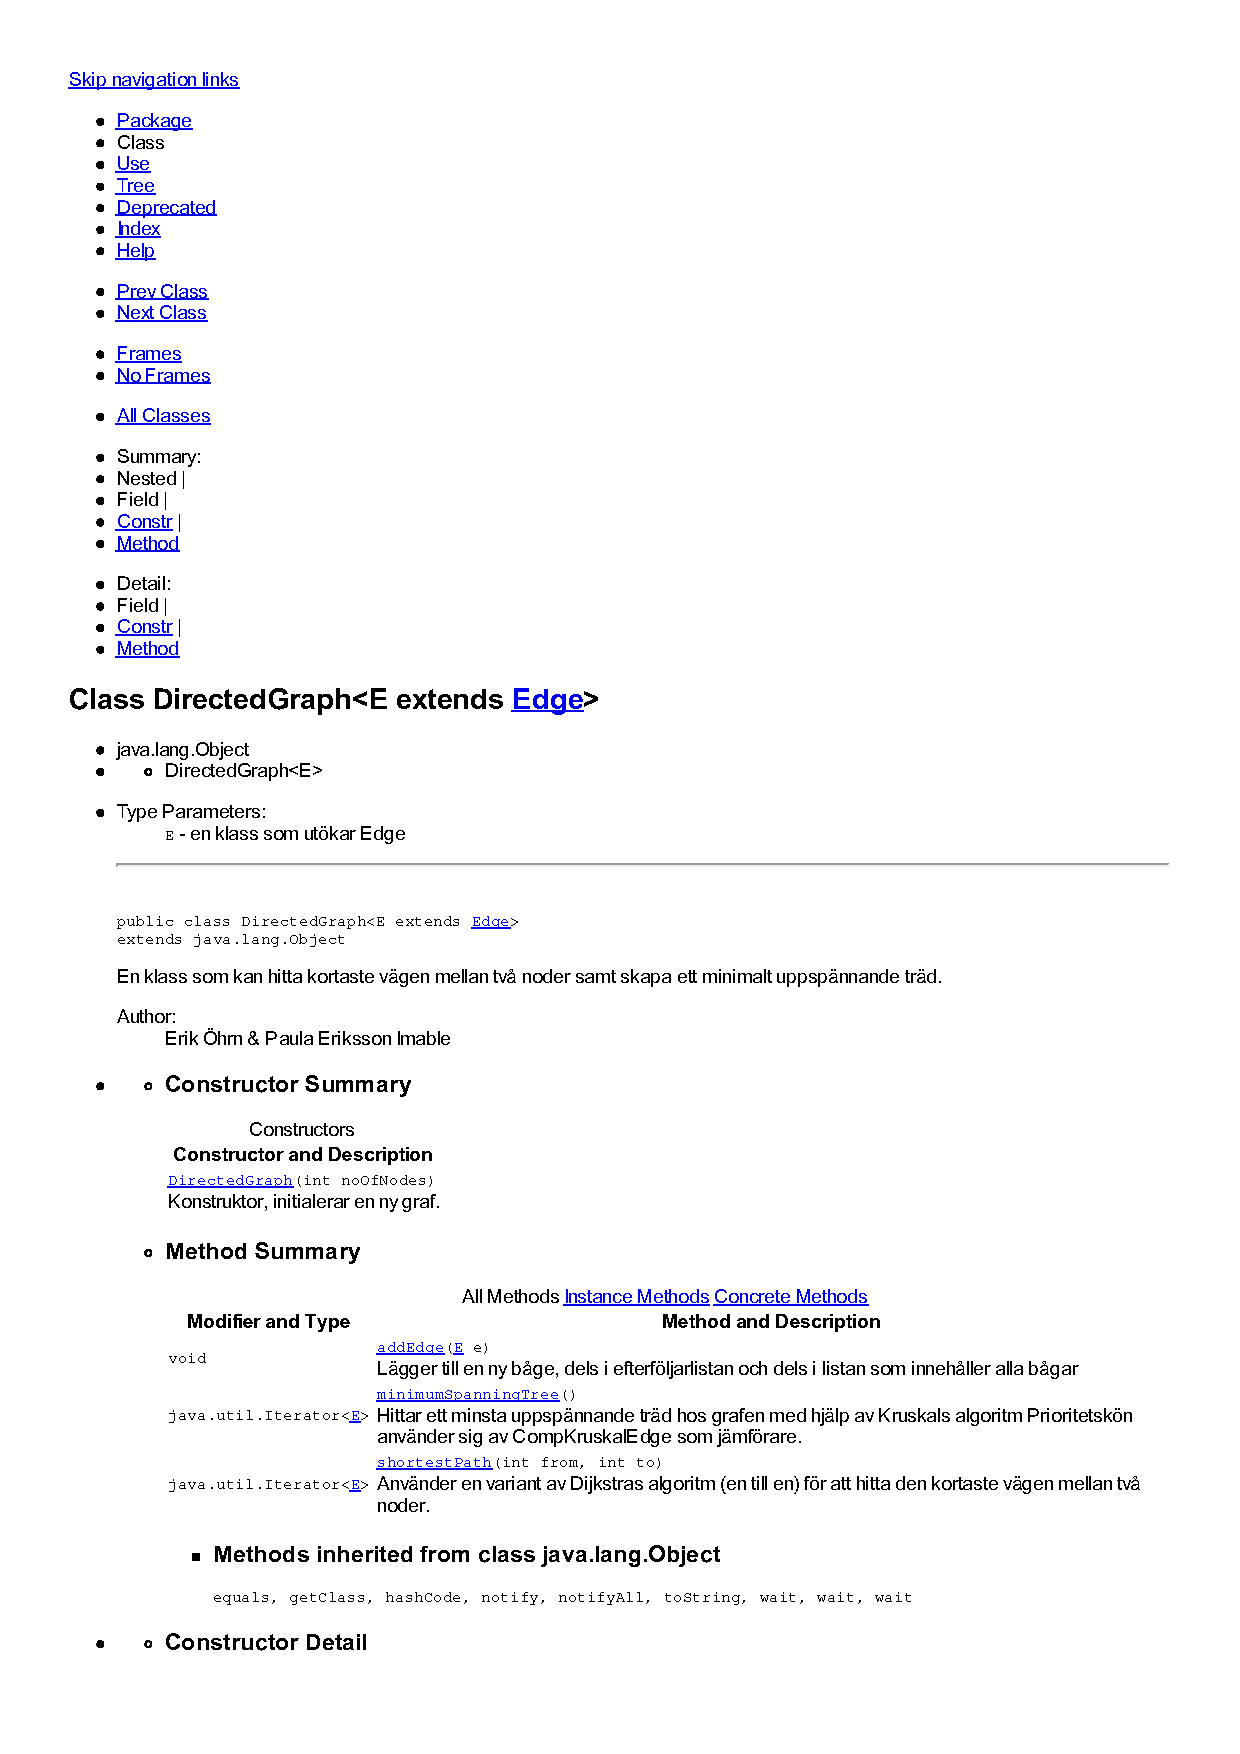
\includepdf[pages=1]{doc/DirectedGraph.pdf}
\includepdf[pages=2]{doc/DirectedGraph.pdf}
\includepdf[pages=3]{doc/DirectedGraph.pdf}
}




\section*{CompDijkstraPath.java}

{
\setbeamercolor{background canvas}{bg=}
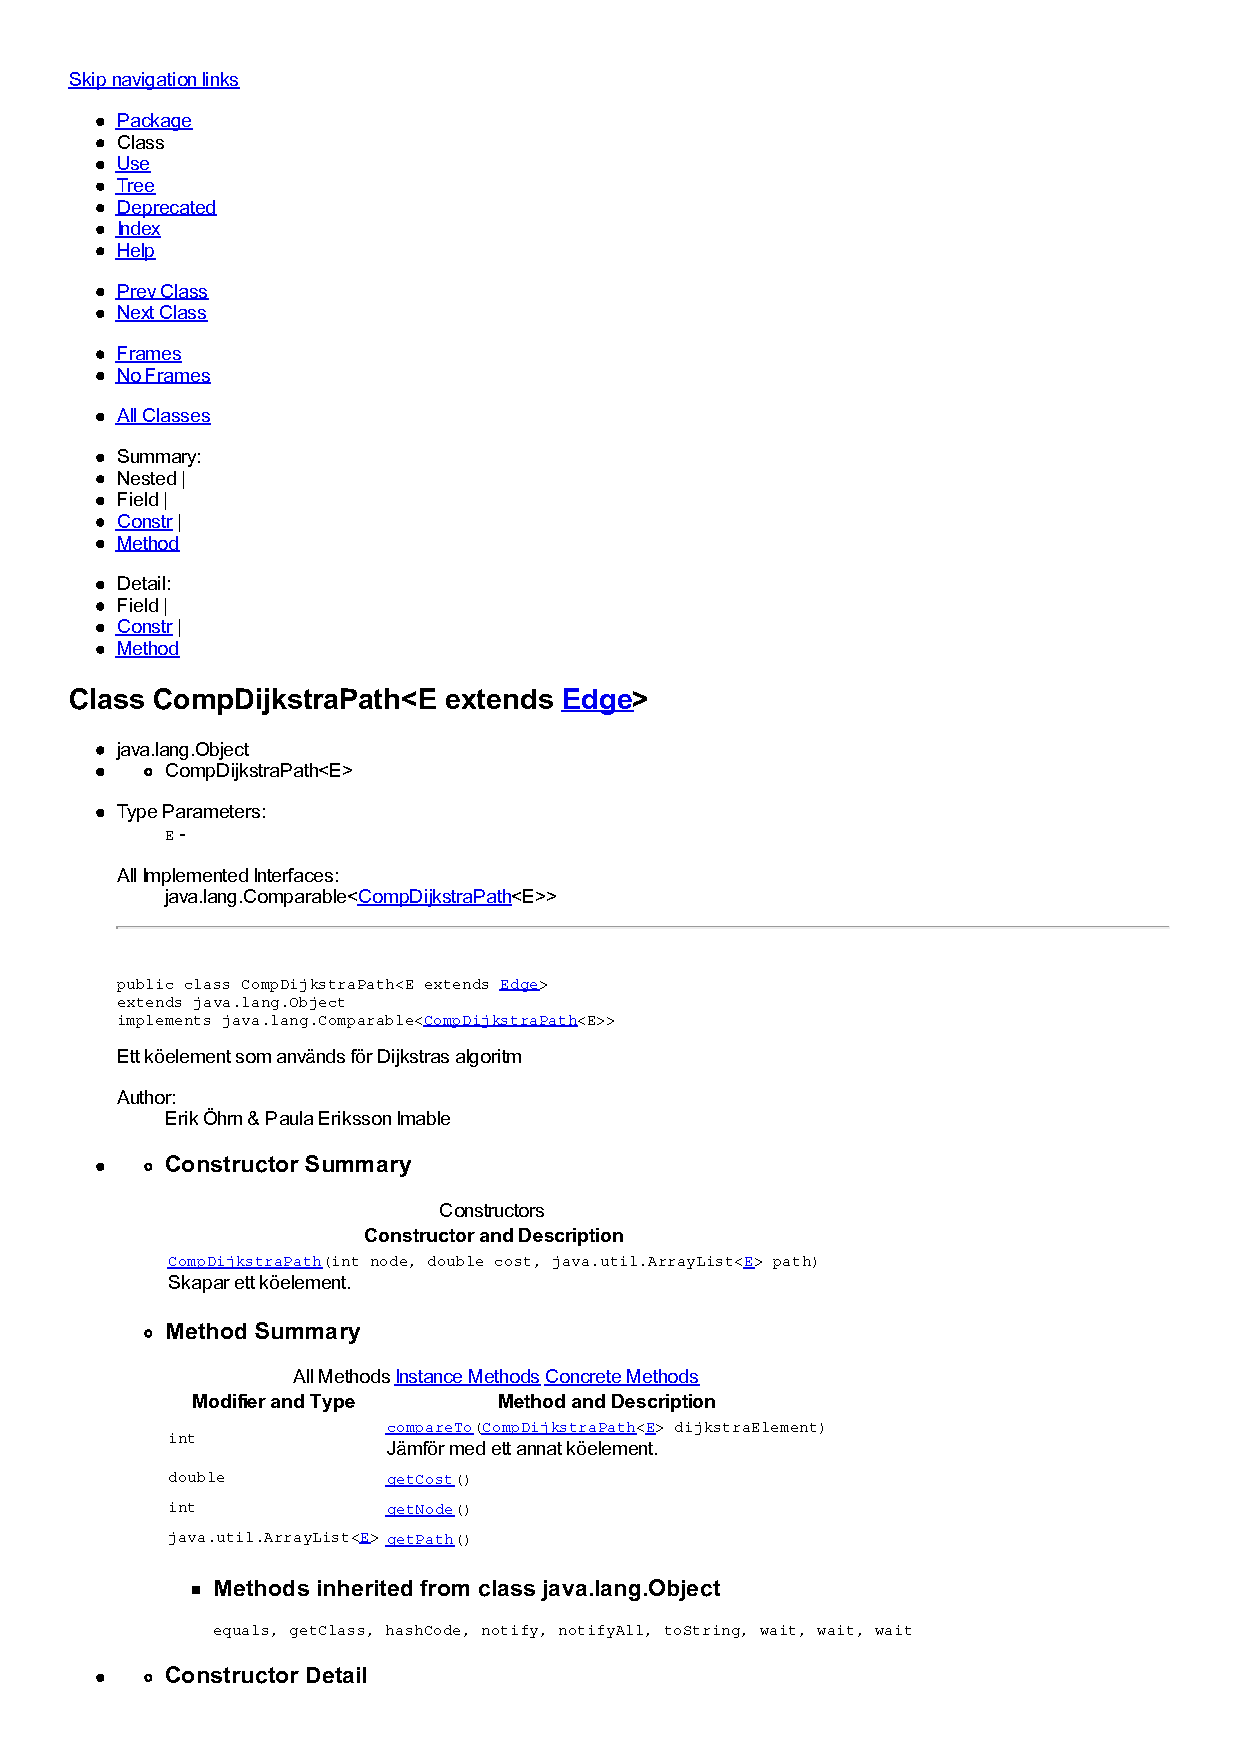
\includepdf[pages=1]{doc/CompDijkstraPath.pdf}
\includepdf[pages=2]{doc/CompDijkstraPath.pdf}
\includepdf[pages=3]{doc/CompDijkstraPath.pdf}
}


\section*{CompKruskalEdge}

{
\setbeamercolor{background canvas}{bg=}
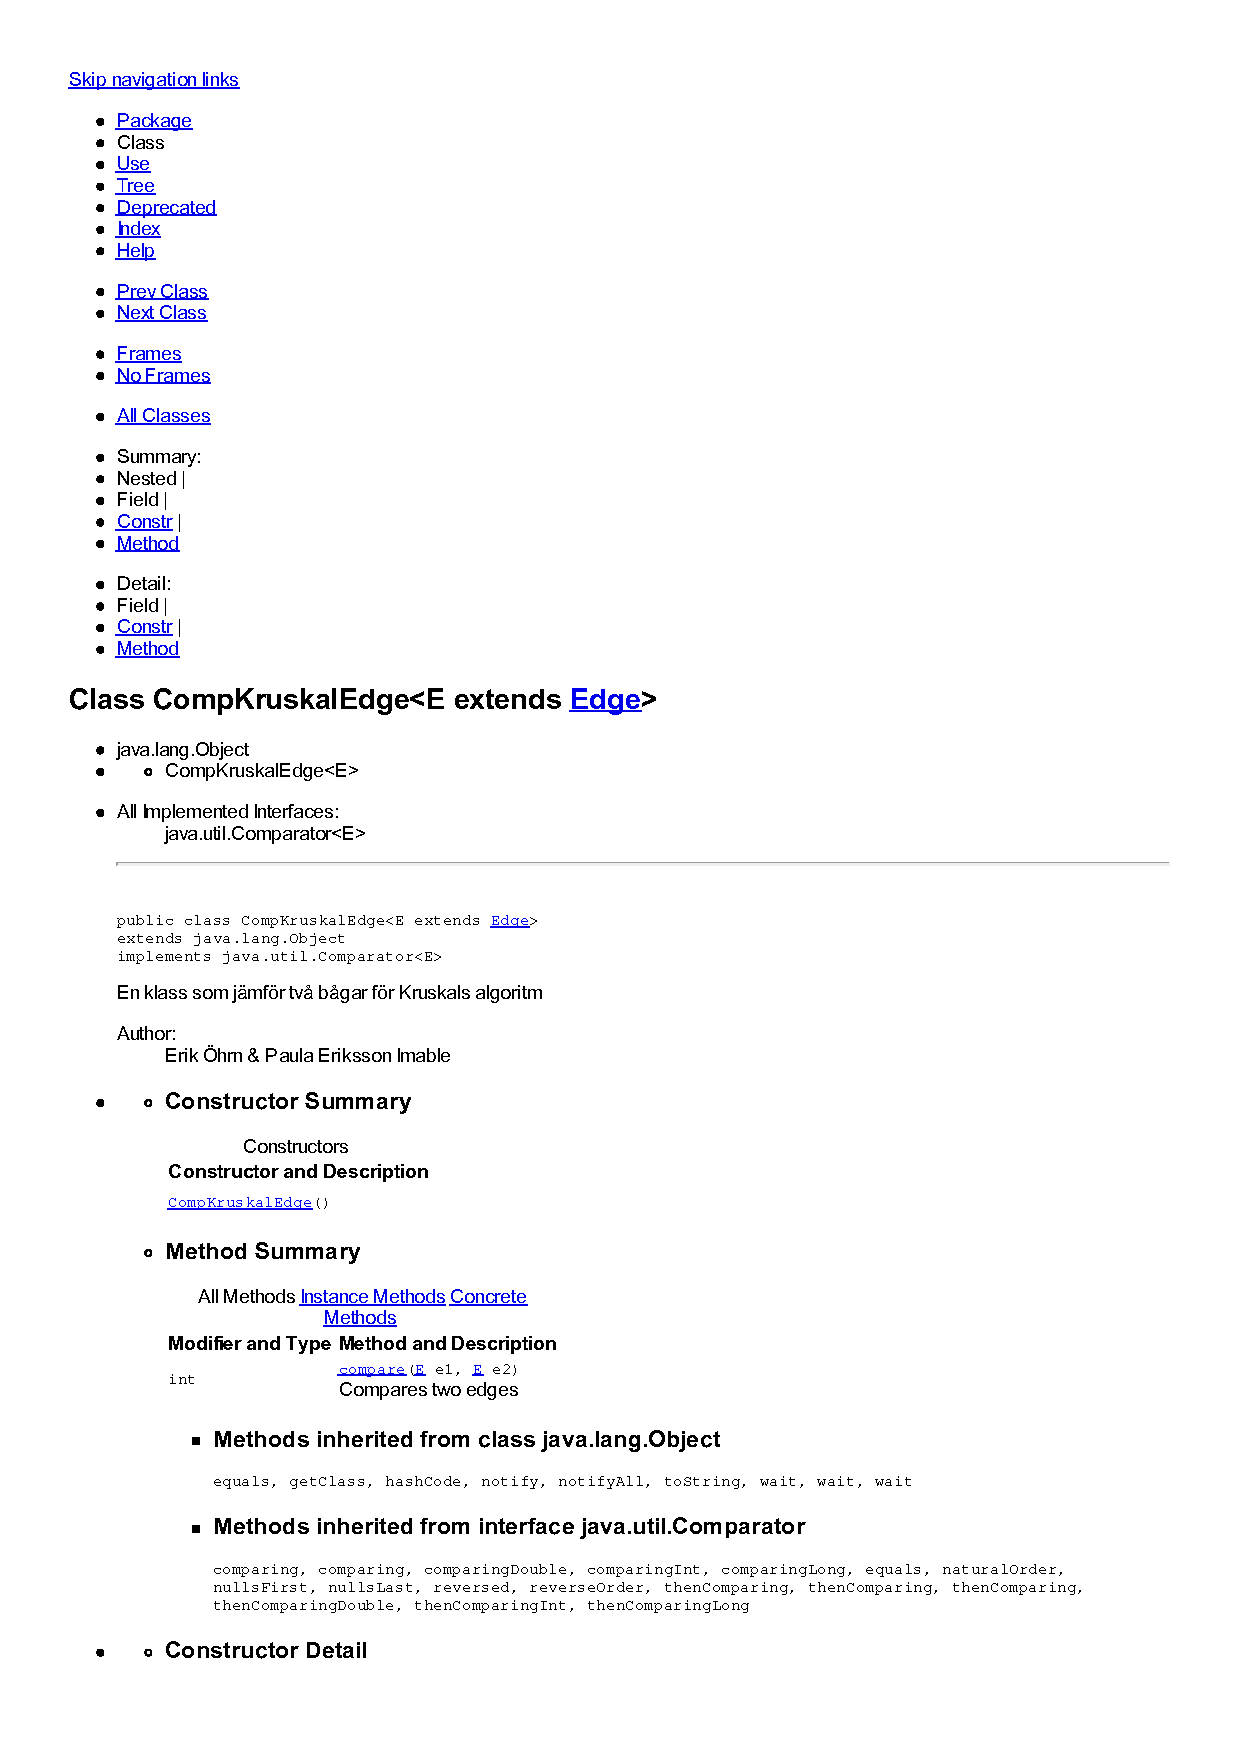
\includepdf[pages=1]{doc/CompKruskalEdge.pdf}
\includepdf[pages=2]{doc/CompKruskalEdge.pdf}
}
\end{document}
